% -----------------------------------------------------
% 下面的附录格式仅供参考,说不定大家到时候时间太紧都
% 没时间写附录了,附录这部分是最开放的哈,想怎么写怎
% 么写,主要内容就是代码和你想放在文章里又没放的东西,
% 比如大型图表等。
% -----------------------------------------------------

\appendix  % 别动!!!

\section{附录:基于Python的统计分析}

\subsection{描述性统计分析}


\begin{lstlisting}[language=Python]
print('Hello World!')
\end{lstlisting}



\subsection{数据可视化}


\begin{lstlisting}[language=Python]
import pandas as pd
import numpy as np
import matplotlib.pyplot as plt
import seaborn as sns

plt.rcParams["font.sans-serif"] = ["SimHei"]
plt.rcParams['font.size'] = 12  # 字体大小
plt.rcParams['axes.unicode_minus'] = False  # 正常显示负号

XXXXXX

plt.figure(figsize=(8, 7))
plt.scatter(df['item_price'], df['ord_qty'], s=10, c='red')
plt.xlabel('item_price')
plt.ylabel('ord_qty')
plt.title("产品价格-需求量散点图")
plt.show()
\end{lstlisting}


\section{附录:基于Python的统计推断}

\subsection{支持向量机}

\begin{lstlisting}[language=Python]
# 支持向量机的实现
\end{lstlisting}


\section{附录:图表(随便放的别当真)}

\begin{figure}[H] 
	\centering %图片居中
	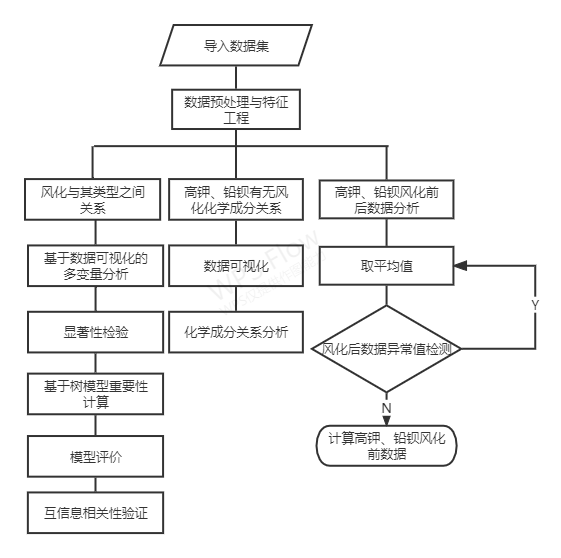
\includegraphics[width=0.7\textwidth]{1.png} %插入图片,[]中设置图片大小,{}中是图片文件名
	\caption{附录图表1} %最终文档中希望显示的图片标题
	\label{Fig.main2} %用于文内引用的标签
\end{figure}

\begin{table}[H]
	\centering
	\begin{tabular}{c c} 
		\toprule[1.5pt]
		符号 & 含义  \\ 
		\midrule[1pt]
		$i=1,i=2$ & 分别表示高钾、铅钡玻璃 \\ 
		$j$ & 表示表中从二氧化硅($SiO_2$)到二氧化硫($SO_2$)中第$j$类化学物质 \\
		$z=1,z=2$ & 分别表示风化前和风化后 \\
		$x_1,x_2,x_3,x_4$ & 分别表示纹饰、类型、颜色、风化表面 \\
		$y_j$ & 表示第$j$类化学物质的含量 \\ 
		$\overline{y_j}$ & 表示第$j$类化学物质的平均含量 \\  
		\toprule[1.5pt]
	\end{tabular}
    \caption{附录图表1}
\end{table} 
